\documentclass[11pt, letterpaper, oneside]{article}

% This document is a simple latex template for reports. It follows the official Lab9K Styleguide, https://github.com/lab9k/Styleguide.

% Packages

\usepackage[dutch]{babel}

\usepackage{geometry}               % Interface to change page dimensions
\usepackage{parskip}                % For better spacing and indenting of paragraphs

\usepackage{graphicx}               % Images
\usepackage[export]{adjustbox}				% Wrap text around figures
\usepackage{fancyhdr}               % Headers and footers
\usepackage{caption}                % Caption

\usepackage{sectsty}                % Manipulate fonts of various sectional headings
\usepackage{enumitem}               % Manipulate enumerate, mdwlist and paralist
\usepackage{makecell}               % Improved tabular layout

\usepackage{url}
\usepackage{hyperref}

\usepackage{fontspec}               % Use own font
\usepackage{anyfontsize}            % Specify font sizes
\usepackage{xcolor}                 % Define own colours

%\usepackage{minted}				% For code snippets

% Configure content of title page

\title{Feedback Linked Open Data\\\mbox{Visit Gent}}
\author{Michiel Derveeuw, Jorg Wieme en Tom Lauwaerts}
\newcommand{\organisation}{Lab9K}
\newcommand{\promotor}{Hans Fraiponts}
\newcommand{\subject}{Rapport over de Linked Open Data van Visit Gent}
\date{6 juli 2018}

% Colour scheme (based on logo)

\definecolor{priColour}{HTML}{026495}              % primary colour
\definecolor{secColour}{HTML}{4a92b8}              % secondary colour

% General configuration and package setup

\geometry{}
\graphicspath{ {figuren/} }    % Map containing all images
\setlength{\headheight}{15pt}

\hypersetup{
	colorlinks=true,
	linkcolor=priColour,
	filecolor=priColour,  
	urlcolor=priColour
}

% Fonts

\setmainfont{Ubuntu}
\setmonofont{Ubuntu}

% General styling

% Use the primary colour for all titles
\sectionfont{\color{priColour}}
\subsectionfont{\color{priColour}}
\subsubsectionfont{\color{priColour}}

% Header
\pagestyle{fancy}
\renewcommand{\headrulewidth}{0pt}
\makeatletter\rhead{\@date}\makeatother

\begin{document}
	\begin{figure}
			
\includegraphics[width=0.27\textwidth,keepaspectratio]{figuren/logo} % Logo of Lab9K
	\end{figure}
	\vspace*{0.35cm}
	
	\makeatletter\fontsize{30pt}{28pt}\selectfont\textcolor{priColour}{\textbf{\@title}}\makeatother
	\newline
	
	\fontsize{11pt}{15pt}\selectfont
	Als we \url{https://visit.gent.be/en/lod/poi} overlopen blijken er enkele problemen te zijn met het json-ld document.
	
	Ten eerste geven alle urls, die als id dienen, steeds een gelijkvormig error bericht terug.
	Zo geeft \url{https://stad.gent/id/place/tourism/7dc10bd0-27d0-4ae5-b72e-a37677141b44}, die het Ibis hotel voorstelt, het volgende terug:
	
	\begin{figure}[!h]
		\centering
		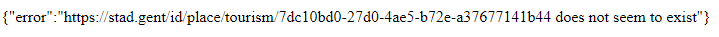
\includegraphics[width=\linewidth]{figuren/error}
	\end{figure}

	Ten tweede bevat de json-ld voor elk \textbf{point of interest} verschillende items (dezelfde id). Deze bevatten bijna volledig dezelfde data, het enige verschil dat we vonden is dat het object van \textbf{scheme:url} naar dezelfde pagina wijst maar in een andere taal. Zo staan er dus veel duplicate triples in het bestand waardoor die onnodig groot wordt.
	
	Dit leidt ons ook naadloos tot de volgende opmerking. Naast een scheme:url heeft een point of interest ook een \\\textbf{foaf:page}, deze lijkt wel uniek (geen taal gespecificeerd). Deze zou dus gerust als id kunnen dienen in plaats van de huidige urls zoals hierboven. (deze zouden dan exact werken als de resource urls van dbpedia)

	Ten derde hebben ContactPoints van een point of interest ook een scheme:url en \\foaf:page, deze verschillen echter en geven beide een 404 statuscode.
	
	Ten vierde hebben timestamps voor elke taal een entry ook al is er geen verschil.
	
	\newpage
	
	Ten slotte kan veel van de data ook niet geïnterpreteerd worden doordat ontologieën niet vermeld zijn of niet bestaan. % TODO uitgebruider verwoorden? druple vermelden?
	Neem het volgende extract uit het json-bestand als illustratie.
	
	\begin{figure}[h]
		\centering
		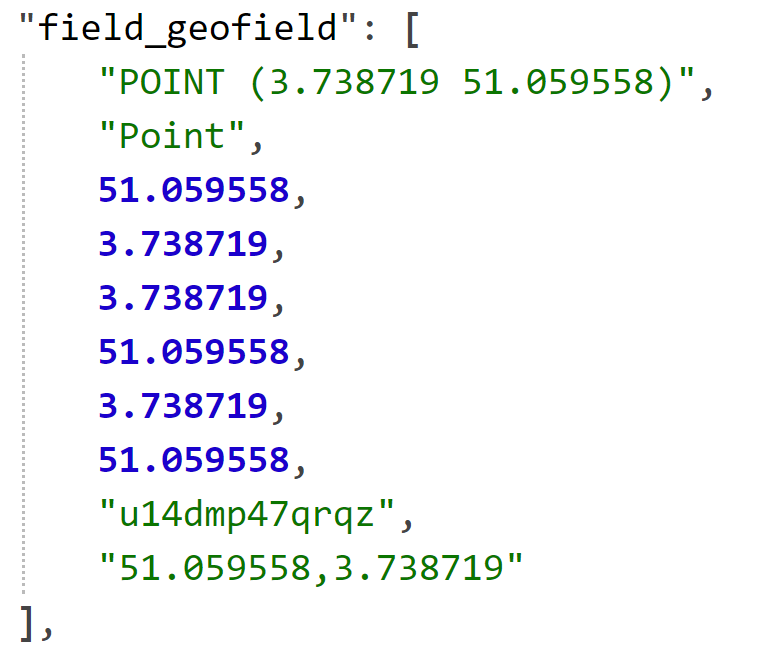
\includegraphics[height=0.5\linewidth]{figuren/field_geofield}
	\end{figure}

	Deze data is om verschillende reden niet te interpreteren. Zo geeft \url{https://schema.org/field_geofield} een 404 terug. Bovendien is het  onmogelijk te weten welke van de 10 verschillende waarden te gebruiken en wat die dan precies voorstellen.
\end{document}